% Harus dimuat terlebih dahulu, digunakan agar file PDF memiliki format karakter yang benar.
% Untuk informasi lebih lanjut, lihat https://ctan.org/pkg/cmap.
\RequirePackage{cmap}

% Format dokumen sebagai paper konferensi menggunakan aturan IEEEtran terbaru (v1.8b).
% Untuk informasi lebih lanjut, lihat http://www.michaelshell.org/tex/ieeetran/.
\documentclass[conference]{IEEEtran}[2015/08/26]

% Format encoding font dan input menjadi 8-bit UTF-8.
\usepackage[T1]{fontenc}
\usepackage[utf8]{inputenc}

% Digunakan untuk tujuan demonstrasi.
\usepackage{mwe}

% Digunakan untuk menampilkan font dengan style yang lebih baik.
\usepackage[zerostyle=b,scaled=.75]{newtxtt}

% Digunakan untuk menampilkan tabel dengan style yang lebih baik.
\usepackage{booktabs}

% Digunakan untuk menampilkan gambar pada dokumen.
\usepackage{graphicx}

% Digunakan untuk menampilkan potongan kode.
\usepackage{listings}
\lstset{
  basicstyle=\ttfamily,
  columns=fixed,
  basewidth=.5em,
  xleftmargin=0.5cm,
  captionpos=b
}

% Digunakan agar backticks (`) dapat dirender pada PDF.
% Untuk informasi lebih lanjut, lihat https://tex.stackexchange.com/a/341057/9075.
\usepackage{upquote}

% Digunakan untuk menyeimbangkan bagian akhir dokumen dengan dua kolom.
\usepackage{balance}

% Digunakan untuk menampilkan pustaka.
\usepackage[square,comma,numbers,sort&compress]{natbib}

% Mengubah format ukuran teks pada natbib.
\renewcommand{\bibfont}{\normalfont\footnotesize}

% Menambah nama penulis ketika menggunakan perintah \citet.
% Untuk informasi lebih lanjut, lihat https://tex.stackexchange.com/a/76075/9075.
\usepackage{etoolbox}
\makeatletter
\patchcmd{\NAT@test}{\else \NAT@nm}{\else \NAT@hyper@{\NAT@nm}}{}{}
\makeatother

% Digunakan untuk melakukan linewrap pada pustaka dengan url yang panjang
% jika terdapat hyphens
\usepackage[hyphens]{url}

% Digunakan untuk menambah hyperlink pada referensi.
\usepackage{hyperref}

% Menonaktifkan warna dan bookmark pada hyperref.
\hypersetup{hidelinks,
  colorlinks=true,
  allcolors=black,
  pdfstartview=Fit,
  breaklinks=true
}

% Digunakan untuk membenarkan hyperref pada gambar.
\usepackage[all]{hypcap}

% Digunakan untuk menampilkan beberapa gambar
\usepackage[caption=false,font=footnotesize]{subfig}

\usepackage{stfloats}

% Tambahkan format tanda hubung yang benar di sini
\hyphenation{
  ro-ket
  me-ngem-bang-kan
  per-hi-tu-ngan
}

\begin{document}

  % Ubah kalimat berikut sesuai dengan judul penelitian.
\title{An LSTM-Based Approach for Two-Step SQL Injection Prevention}

% Ubah kalimat-kalimat berikut sesuai dengan nama, institusi, alamat dan kontak penulis.
\makeatletter
\newcommand{\linebreakand}{%
  \end{@IEEEauthorhalign}
  \hfill\mbox{}\par
  \mbox{}\hfill\begin{@IEEEauthorhalign}
}
\makeatother

\author{
  \IEEEauthorblockN{1\textsuperscript{st} Tomy Tjandra}
  \IEEEauthorblockA{\textit{Computer Science and Information Engineering} \\
    \textit{National Taiwan University of Science and Technology}\\
    Taipei, Taiwan\\
    M11115806@mail.ntust.edu.tw}
  \and
  \IEEEauthorblockN{2\textsuperscript{nd} Charles Chang}
  \IEEEauthorblockA{\textit{Computer Science and Information Engineering} \\
    \textit{National Taiwan University of Science and Technology}\\
    Taipei, Taiwan\\
    M11115802@mail.ntust.edu.tw}
  \linebreakand
  \IEEEauthorblockN{3\textsuperscript{rd} Glenn Nicholas}
  \IEEEauthorblockA{\textit{Computer Science and Information Engineering} \\
    \textit{National Taiwan University of Science and Technology}\\
    Taipei, Taiwan\\
    M11115812@mail.ntust.edu.tw}
  \and
  \IEEEauthorblockN{4\textsuperscript{th} Darwin Gunawan}
  \IEEEauthorblockA{\textit{Computer Science and Information Engineering} \\
    \textit{National Taiwan University of Science and Technology}\\
    Taipei, Taiwan\\
    M11115808@mail.ntust.edu.tw}
}

% Digunakan untuk menampilkan judul dan deskripsi penulis.
\maketitle

  % Mengubah keterangan `Abstract` ke bahasa indonesia.
% Hapus bagian ini untuk mengembalikan ke format awal.
\renewcommand\abstractname{Abstrak}

\begin{abstract}

  % Ubah paragraf berikut sesuai dengan abstrak dari penelitian.
  Pada penelitian ini kami mengajukan \lipsum[1][1-12]

\end{abstract}

% Mengubah keterangan `Index terms` ke bahasa indonesia.
% Hapus bagian ini untuk mengembalikan ke format awal.
\renewcommand\IEEEkeywordsname{Kata kunci}

\begin{IEEEkeywords}

  % Ubah kata-kata berikut sesuai dengan kata kunci dari penelitian.
  Roket, Anti-gravitasi, Energi, Angkasa.

\end{IEEEkeywords}


  % Ubah bagian berikut sesuai dengan konten-konten yang akan dimasukkan pada dokumen
  % Ubah judul dan label berikut sesuai dengan yang diinginkan.
\section{Introduction}
\label{sec:introduction}

% Ubah paragraf-paragraf pada bagian ini sesuai dengan yang diinginkan.
\par SQL injection (SQLi) is an attack technique that allows malicious actors to inject code on a database server through a web application's input field \cite{7395166}. This technique can be destructive to a database, making malicious actors capable of gaining access to sensitive information, destroying data, or understanding the whole system.
\par The prevention of SQLi attacks is critical for web developers and security professionals. According to OWASP 2021 \cite{OWASP}, SQLi is listed as the top 3 out of 10 most serious web application security risks with a max incident rate of 19\% and an average incidence rate of 3.37\%. The common practice of SQLi attacks prevention is to use input validation and sanitization, which directly detect and filter out malicious input before it gets processed by the database server. But even these techniques still have limitations in handling complex SQLi and need more effort to update the techniques to keep handling the SQLi since malicious actors always find ways to break the security.

\par In this modern era, machine learning exists to be a promising alternative for detecting and preventing SQLi attacks. SQLi attacks from the past can be used as a dataset for machine learning to learn and become capable of preventing SQLi attacks in the future. With this approach, machine learning can adapt to new types of SQLi attacks by learning and evolving, making malicious actors have difficulty bypassing the database server. Furthermore, this approach may handle more complex and shady input from malicious actors rather than only using the common practice.

\par In this report, we will implement two-step SQLi prevention, which combines keyword filtering with blacklist and machine learning prediction with LSTM. Besides evaluating the model's predictive performance, we will also review the prediction time by comparing it with various classical machine learning algorithms.

\par This report is organised as follows. Section \ref{sec:related-works} will discuss three related state-of-the-art approaches in this area. Section \ref{sec:prerequisites} will provide the key concepts related to this project. Section \ref{sec:proposed-design} will describe our overall approach and delve more into our proposed two-step prevention. In Section \ref{sec:experiment-setup}, we will describe the experimental setup for our approach. In Section \ref{sec:result}, we will present our experiments' results and compare them to the state-of-the-art approaches listed in Section II. Lastly, in Section \ref{sec:conclusion}, we will conclude this paper.
  % Ubah judul dan label berikut sesuai dengan yang diinginkan.
\section{Related Works}
\label{sec:related-works}

% Ubah paragraf-paragraf pada bagian ini sesuai dengan yang diinginkan.

\par Many researchers have researched the method of detecting SQLi attacks using machine learning, with each proposing new methods and applying different algorithms. With many types of research already published with the same goal, we will review their approach and methodology in this section.
\par Li et al. \cite{8854182} proposed a deep forest-based SQLi method framework. Their framework consists of two stages: offline training and online testing. Both stages are similar in that they involve preprocessing, feature extraction, and generating vectors. The offline stage includes a data collection step, while the online stage must output a result (malicious or non-malicious) using the trained model. The Adaptive Deep Forest Model (ADF) is the main component of their algorithm. Compared to other algorithms, this has the advantage of fully utilizing the information because the model's depth is sufficiently complex, and vectors are processed by layers while being able to complete intra-layer transformation. The ADF also allows the model to ignore parts of the feature vectors that may affect the model. Li et al. also introduced the AdaBoost algorithm, which improves the ability of the deep forest model to self-adjust. Within each level of the deep forest, the weights of the features are updated based on the classification error rate. This is particularly useful in solving the imbalanced distribution of multi-type samples. The ADF allows the model parameters to be adjusted automatically in the training process, which improves detection accuracy.
\par Hasan, Balbahaith, and Tarique \cite{8959617}, similar to ours and the previous work's approach, used a feature extractor where the extracted features are used to determine whether a query is malicious or not. Their proposed system is placed between the application and the system to evaluate incoming queries before forwarding them to the database. To decide which algorithms are best suited for their system, they evaluated the performance of different classifiers before finally choosing the Ensemble Boosted and Bagged Trees classifiers because they had the highest accuracy. The researchers of this paper also developed a graphical user interface (GUI) for users to enter queries and have them classified by their system. Although this paper compares the performance of 23 algorithms, the dataset size is small (616 statements), and the final accuracy is also taken from the training data, so it does not show a good representation of the actual result.
\par Li et al. \cite{8616823} discuss a method called long short-term memory (LSTM) that has been applied in our paper and is heavily used in deep learning. Like previous works, LSTM is used as a feature extractor and trains the classifiers for SQLi attacks. In this paper, the feature vector used is called word2vec because it yielded better results than the bag-of-words approach. In our paper, we implemented the term frequency-inverse document frequency (TF-IDF). This paper also made use of six datasets, with the first one being used for training. From the data split of all the datasets, Dataset 3 has a similar data structure to ours. Therefore, we can compare the results between our proposed method and theirs.
\par With many different approaches for SQLi detection, most have a similar approach where it starts with string matching or feature extraction. However, with the increase in technology literacy, meaning that hackers are becoming more intelligent, security must also become more advanced. In this paper, we propose a two-step approach by incorporating keyword filtering and model prediction within one architecture.


  % Ubah judul dan label berikut sesuai dengan yang diinginkan.
\section{Key Concepts}
\label{sec:prerequisites}

% Ubah paragraf-paragraf pada bagian ini sesuai dengan yang diinginkan.

\subsection{SQL Injection (SQLi)}
\label{subsec:SQLi}
\par SQLi is a type of cyber-attack in which a malicious actor injects code into a website's database through an input field to gain unauthorized access to sensitive information. This attack is particularly dangerous because it allows attackers to bypass security measures and gain access to sensitive data such as customer information or proprietary business data. SQLi attacks have become more common in recent years as more companies move their operations online. This is partly because many websites and web-based applications are not protected against this attack. To protect against SQLi, a company or organization should take many measures to secure its website and database. The code below shows a sample of an SQLi query where the malicious user tries to get admin access by making the password equal to TRUE.

% Contoh pembuatan potongan kode.
\begin{lstlisting}[
  language=SQL,
  caption={Sample of SQL Injection code},
  label={lst:SQLi}
]
SELECT * 
FROM users 
WHERE username = 'admin' AND password = '' OR '1' = '1'
\end{lstlisting}

\subsection{Keyword Filtering}
\label{subsec:keyword-filtering}
\par One of the most common methods to prevent SQLi is to use keyword filtering, which involves setting up a filter that does not allow specific keywords or commands to be entered into an input field. For example, suppose a website does not have SQL commands such as "SELECT", "FROM", "WHERE", and "INSERT" using regex, ensuring that user-entered data does not contain potentially harmful codes or characters. In that case, the filter automatically blocks any attempts to enter other types of commands or code. This makes it much more difficult for attackers to inject malicious code into the database because the input data is checked if it is in the keyword filtering list, if it is, then it will not be executed.
\par However, it is important to note that keyword filtering is not a foolproof method for protecting against SQLi. This is because attackers can often bypass keyword filters by using alternative syntax or encoding their code in a way that is not detected by the filter. Therefore, keyword filtering should be used in conjunction with other security measures, such as adding a machine learning model to predict if a given input is malicious or not to provide a more comprehensive defense against SQLi attacks.

\subsection{Long Short-Term Memory (LSTM)}
\label{subsec:LSTM}
\par LSTM is a type of Recurrent Neural Network (RNN) developed by Hochreiter and Schmidhuber in 1997 \cite{10.1162/neco.1997.9.8.1735}. One key advantage of LSTMs over traditional RNNs is their ability to store and access information over longer periods of time, thanks to the use of "memory cells" that can store and update information as needed. This allows LSTMs to handle better tasks that require considering context from earlier in the input sequence and tasks with long-term dependencies.
\par Like traditional RNNs, LSTMs can also process input sequences in both forward and backward directions. This allows the network to consider contextual information from past and future time steps when processing input sequences.
\par LSTMs have been successfully applied to various tasks, including language translation, speech recognition, and text classification. Considering the state-of-the-art approach of using LSTM on natural language processing tasks, we use a many-to-one LSTM model to classify an input query as either malicious or safe.

  % Ubah judul dan label berikut sesuai dengan yang diinginkan.
\section{Proposed Design}
\label{sec:proposed-design}

% Ubah paragraf-paragraf pada bagian ini sesuai dengan yang diinginkan.

% Contoh input beberapa gambar pada halaman.
\begin{figure*}
  \centering
  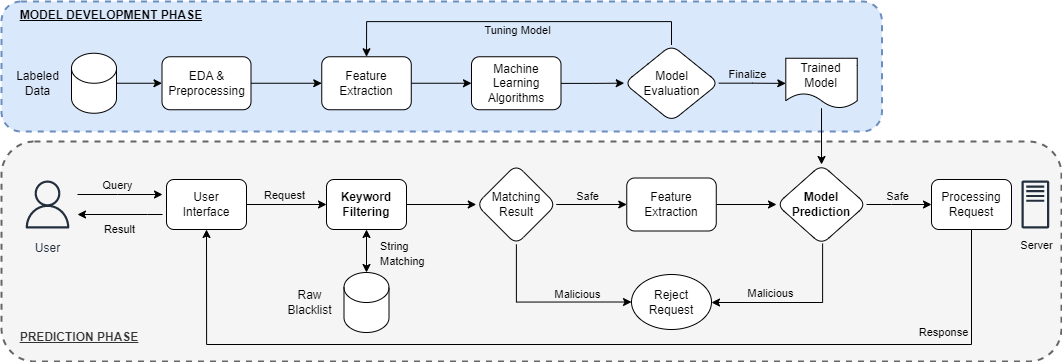
\includegraphics[width=.82\textwidth]{image/SQLI-Final.drawio.png}
  \caption{Design Workflow}
  \label{fig:proposed-workflow}
\end{figure*}

\par Figure \ref{fig:proposed-workflow} shows our proposed design, which separates the workflow into two phases. The model development phase aims to build a machine-learning model with the best predictive performance and the least prediction time. In the prediction phase, we implement the two-step prevention approach by combining keyword filtering and model prediction to prevent SQLi attacks.

\par The first step of the model development phase is to gather labeled data and an indicator of whether it is a malicious or safe query. Exploratory Data Analysis (EDA) is performed to understand the data better and decides the appropriate hyperparameters for the model. Preprocessing refers to the query cleansing step. Below, we provide an example of a query being cleansed consecutively:

\begin{itemize}[
    \setlength{\IEEElabelindent}{\dimexpr-\labelwidth-\labelsep}% Wrapping of text beyond first line of \item
    \setlength{\itemindent}{\dimexpr\labelwidth+\labelsep}% identation for each new \item
    \setlength{\listparindent}{\parindent}% Restore regular paragraph indentation
  ]
  \item Case folding: convert all text queries to lowercase since uppercase, and lowercase tokens have the same meaning. Example: 23" and 65 = 65 || chr (113) and "0x77" like "0x77
  \item Punctuation padding: insert white space before and after each punctuation to separate from alphanumeric characters, and each punctuation can be treated as one token. Example: 23 " and 65 = 65 | | chr ( 113 ) and " 0x77 " like " 0x77
  \item Numeric mapping: numeric values are too specific to be considered a single token, so they are mapped into each corresponding tag. There are three tags: <NUM> for regular numeric, <HEX> for hexadecimal, and <ASCII\_DEC> for a numeric followed by a char function. Example: <NUM> " and <NUM> = <NUM> | | chr ( <ASCII\_DEC> ) and " <HEX> " like " <HEX>
  \item Tokenizing: split the cleaned query into a list of tokens, using a single space as the separator. Example result: 19 tokens
\end{itemize}

\par The cleaned queries are converted into vector representation so that the model can compute numerically. The feature extraction technique for machine learning is TF-IDF, while a regular embedding layer is used for deep learning. The features are then fitted into several supervised machine learning algorithms (including LSTM). The model is evaluated using cross-validation and fine-tuned by adjusting the hyperparameters until it is optimized enough in terms of predictive performance and prediction time.

\par During the prediction phase, the query input by the user is matched to the static raw blacklist in the database. The user's request is considered malicious if a match is found in the blacklist. If it is considered safe, it is continued as input to the machine learning model to be predicted. Notice that the exact feature extraction step still has to be performed to represent the query using vector representation. The server will reject the user's request if the model predicts the query is malicious. If the query passes both keyword filtering and model prediction, the server will process it and return the result to the user via the user interface. The decision-making during this phase can be summarized using a logical OR operator shown in Table \ref{tab:decisionmaking}.

\begin{table}
  \caption{Decision making during the prediction phase}
  \label{tab:decisionmaking}
  \centering
  \begin{tabular}{lll}
    \toprule
    Keyword Filtering & Model Prediction & Final Decision  \\
    \midrule
    Malicious      & Malicious      & Malicious     \\
    Malicious      & Safe      & Malicious     \\
    Safe      & Malicious      & Malicious     \\
    Safe      & Safe      & Safe     \\
    \bottomrule
  \end{tabular}
\end{table}
  % Ubah judul dan label berikut sesuai dengan yang diinginkan.
\section{Experiment Setup}
\label{sec:experiment-setup}

% Ubah paragraf-paragraf pada bagian ini sesuai dengan yang diinginkan.

\subsection{Model Development Phase}
\label{subsec:model-development-phase}
\par We use a public dataset available on Kaggle, comprising 30,905 raw queries of SQLi attacks and benign traffic from different websites \cite{SQLiDataset}. With a 63:37 ratio of safe to malicious query, we consider this case as an imbalanced dataset. In reality, a malicious query occurs less than a safe query. Thus, using the F1 score to evaluate the model is more suitable for this case. A stratified train-test split with a ratio of 80:20 is performed on the data.
\par A fixed-length sequential data is required to train the LSTM. Based on Figure \ref{fig:eda_violinplot_n_token_query}, we set the maximum length of a query to be 30 tokens, which satisfies more than 90\% of the training data. If a query is more than 30 tokens, the query will be pre-truncated, and if less than 30 tokens, the query will be pre-padded with zero vectors. Also, several tokens only occur once in the dataset, which can be assumed as noise tokens. Hence, based on Figure \ref{fig:eda_lineplot_token_cutoff_freq.png}, we set the cut-off frequency to two. In other words, all tokens that only occur once will be treated as an out-of-vocabulary token.

\begin{figure} [ht]
  \centering
  % Ubah sesuai dengan nama file gambar dan ukuran yang akan digunakan.
  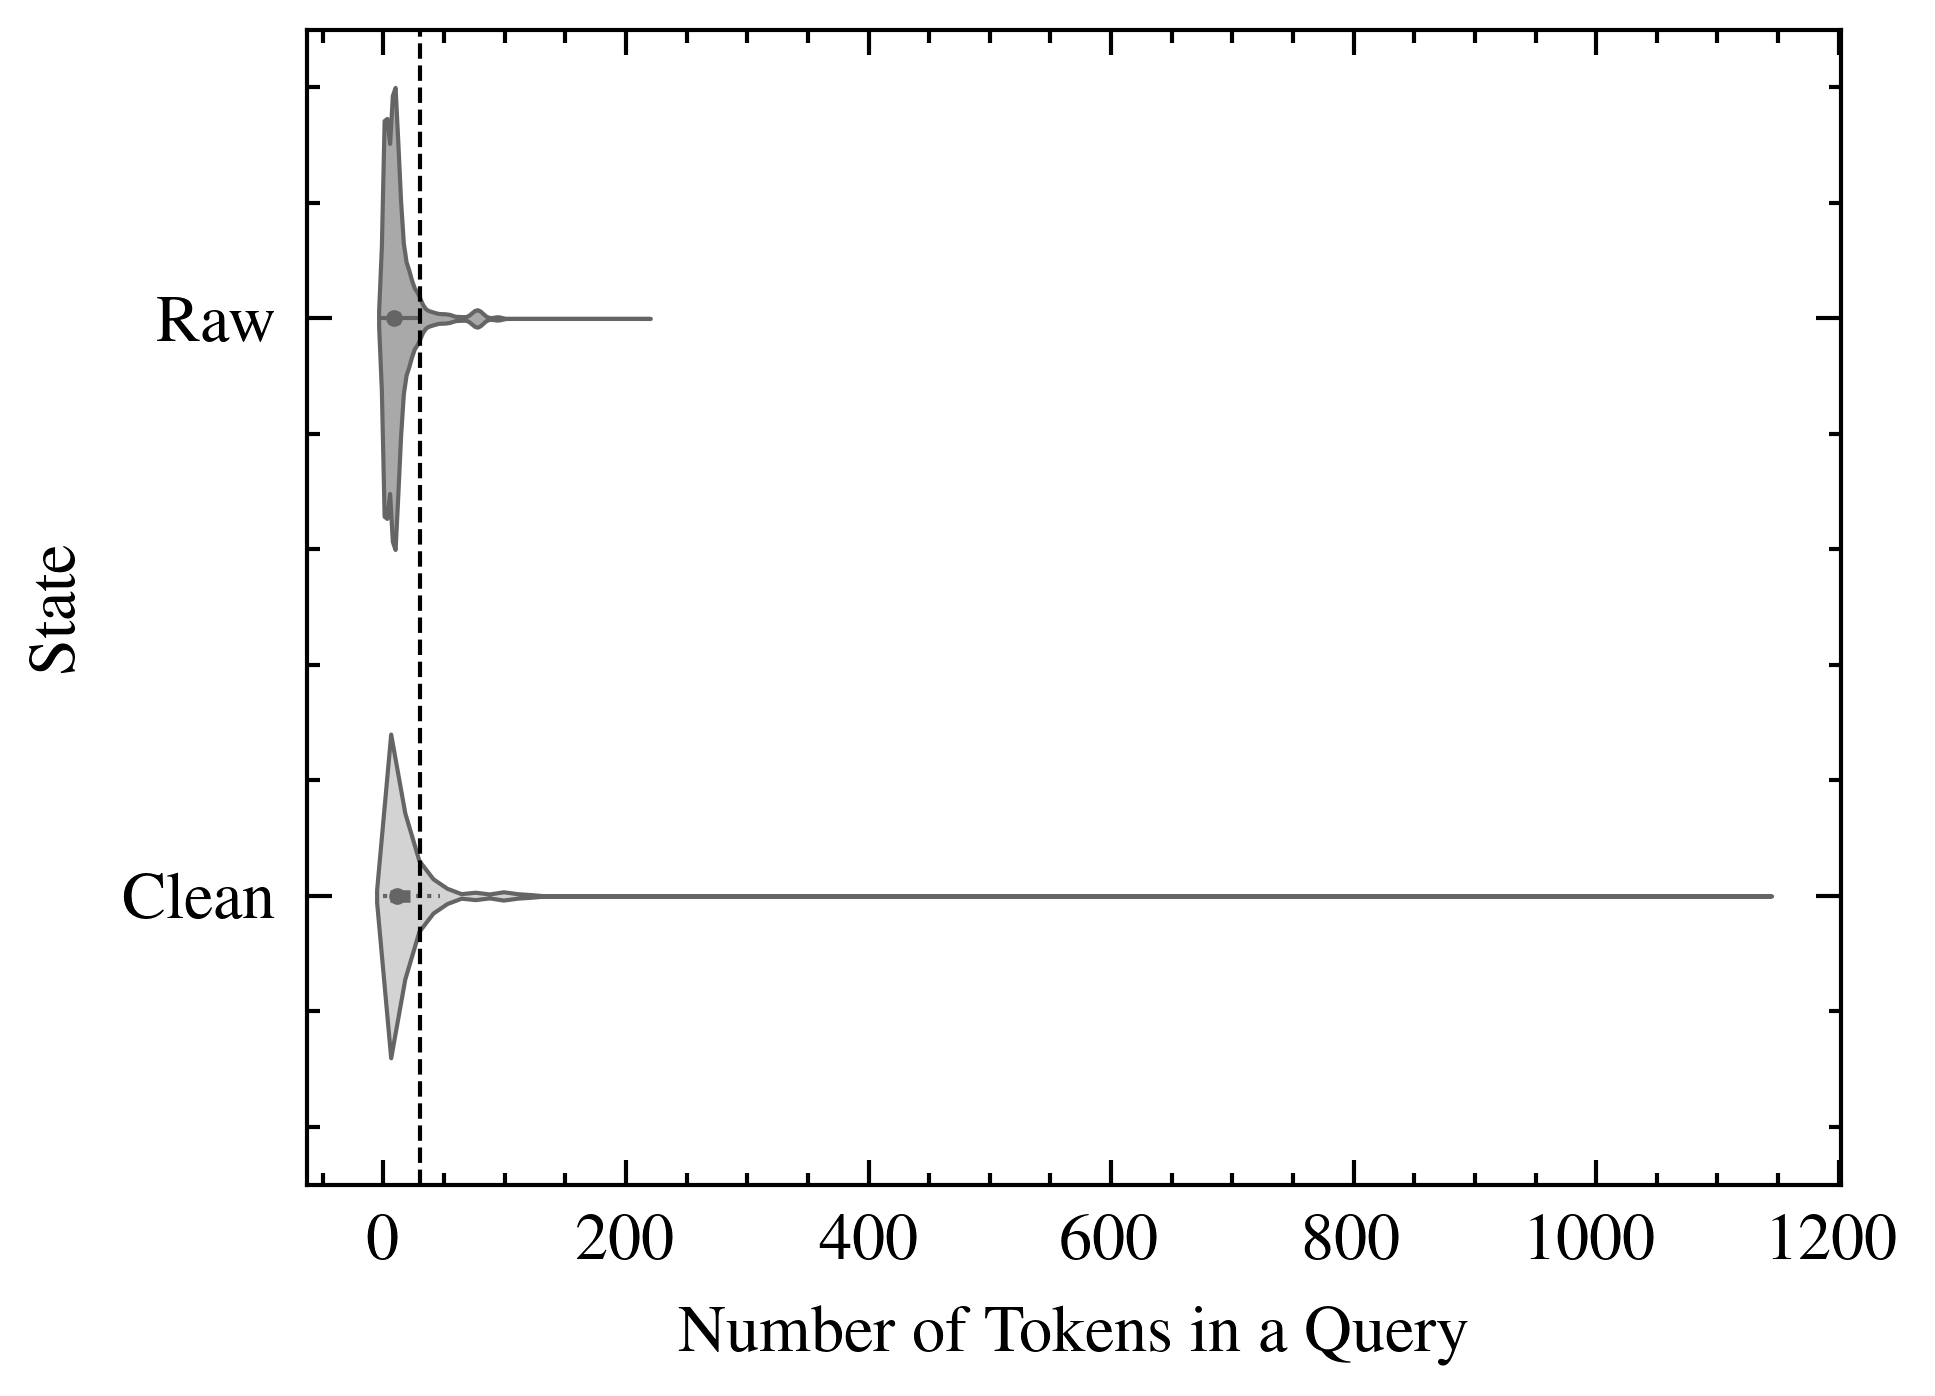
\includegraphics[width=0.4\textwidth]{image/eda_violinplot_n_token_query.png}

  % Ubah sesuai dengan keterangan gambar yang diinginkan.
  \caption{The distribution of the number of tokens in a query}
  \label{fig:eda_violinplot_n_token_query}
\end{figure}

\begin{figure} [ht]
  \centering
  % Ubah sesuai dengan nama file gambar dan ukuran yang akan digunakan.
  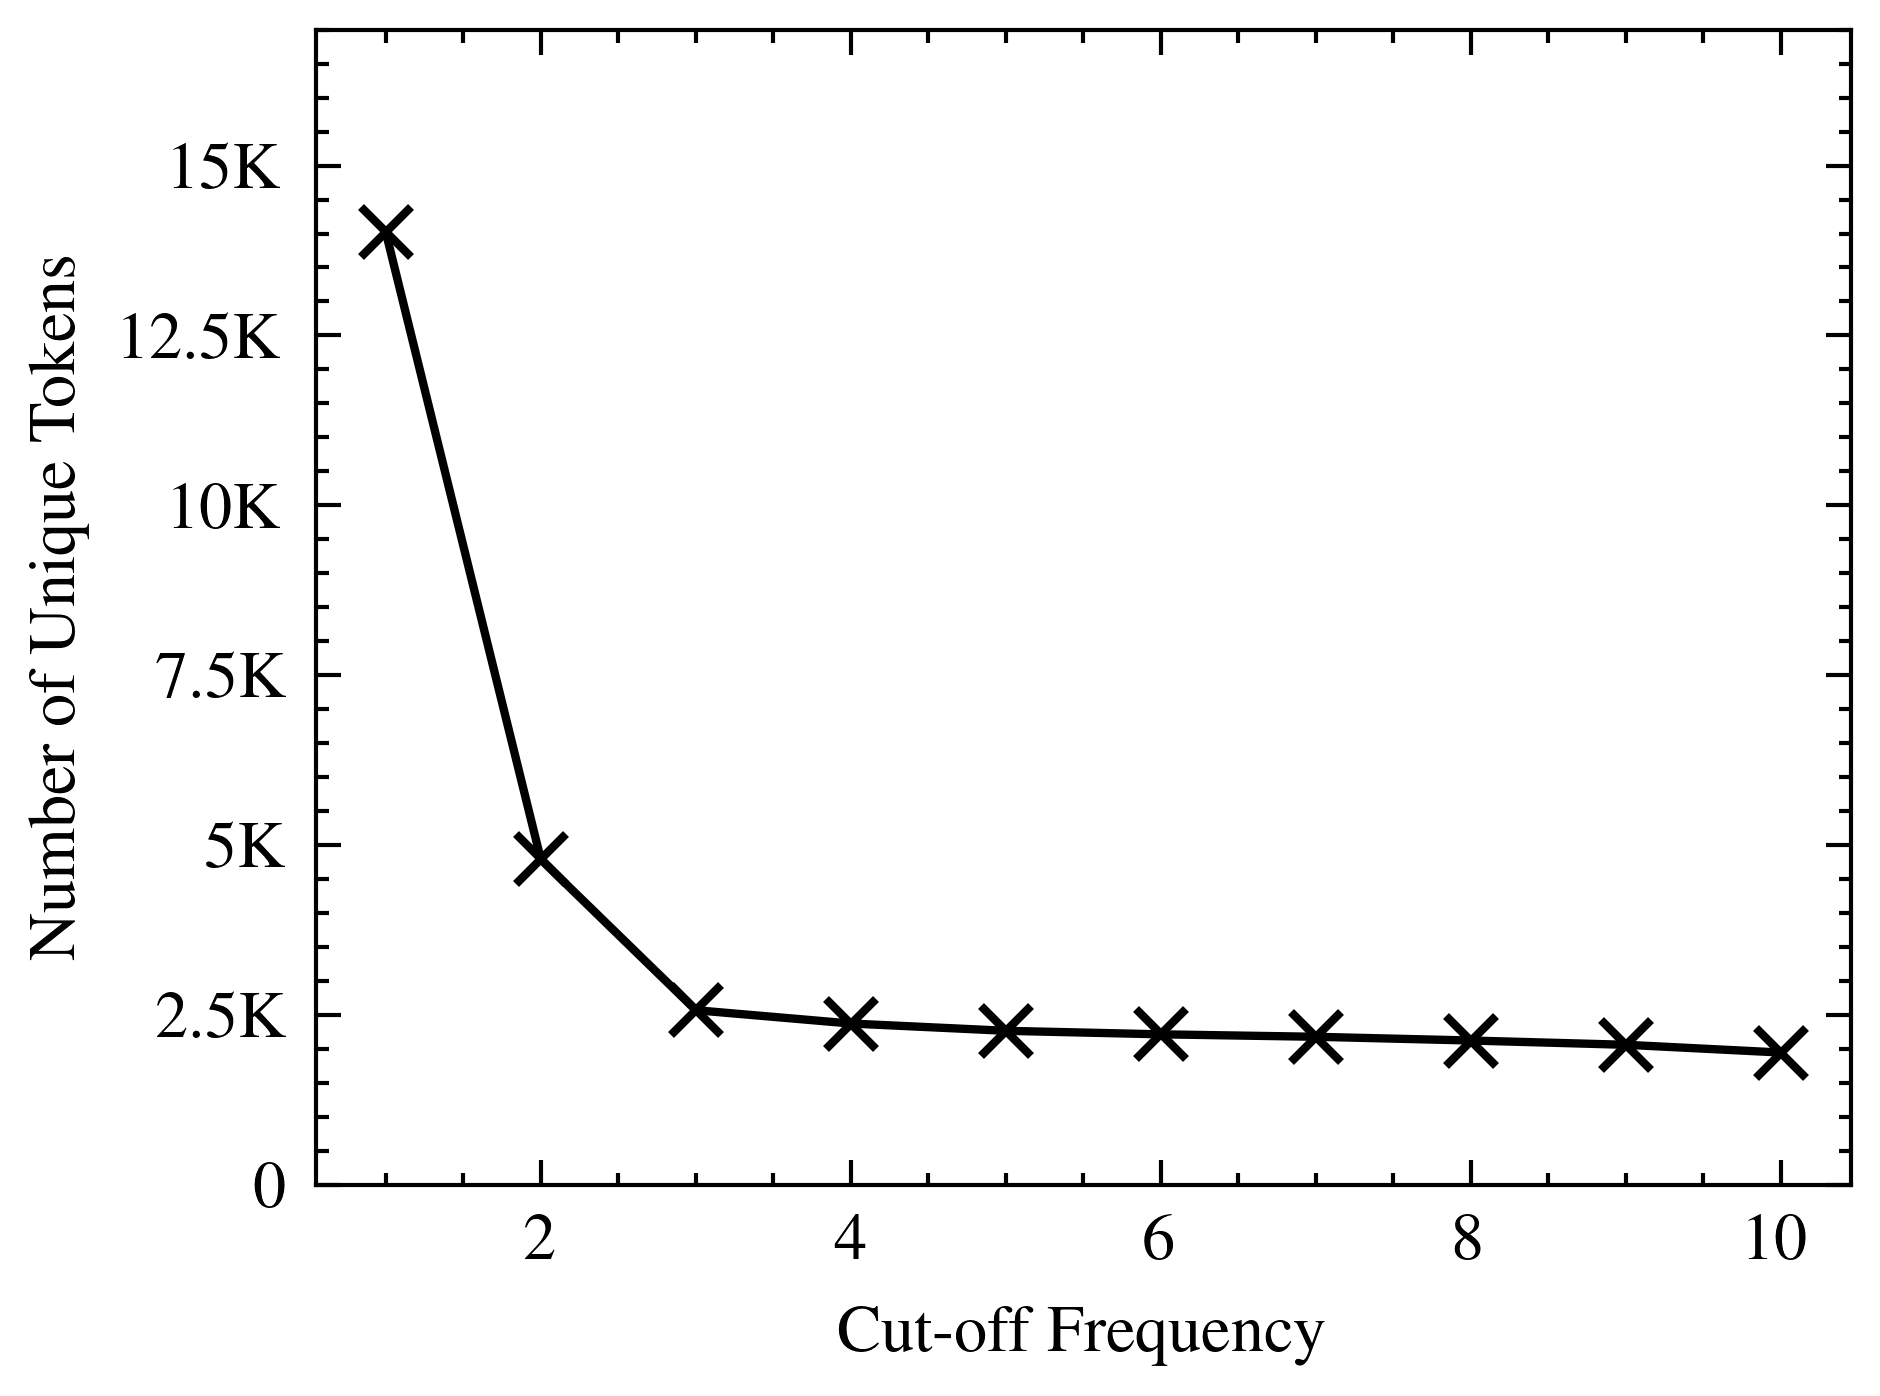
\includegraphics[width=0.35\textwidth]{image/eda_lineplot_token_cutoff_freq.png}

  % Ubah sesuai dengan keterangan gambar yang diinginkan.
  \caption{Token cut-off frequency}
  \label{fig:eda_lineplot_token_cutoff_freq.png}
\end{figure}

\par The "best" LSTM model is obtained by searching the hyperparameter out of 18 combinations (shown in Table \ref{tab: hyperparameter-lstm}) that achieve the highest mean F1 score in the validation data using 5-fold cross-validation. For comparison, we also trained the data using ten supervised machine-learning algorithms using default hyperparameters from scikit-learn \cite{scikit-learn}:
\begin{itemize}[
    \setlength{\IEEElabelindent}{\dimexpr-\labelwidth-\labelsep}% Wrapping of text beyond first line of \item
    \setlength{\itemindent}{\dimexpr\labelwidth+\labelsep}% identation for each new \item
    \setlength{\listparindent}{\parindent}% Restore regular paragraph indentation
  ]
  \item Linear classifier: Logistic regression, Linear discriminant analysis, SVM linear
  \item Non-linear classifier: KNN, Naive Bayes, SVM using RBF kernel
  \item Tree-based model: Decision tree (depth = 50), Random forest (depth = 50), Ada boost, Gradient boost
\end{itemize}

\par Each model's prediction time is also considered because, in a real-world application, the model has to be as fast as possible to predict the user query. Ideally, we want a predictive model with a maximum F1 score and minimum prediction time. We measured the prediction time in milliseconds per query by predicting the validation data during 5-fold cross-validation. Table \ref{tab: specifications} shows the hardware and software specifications used for our experiments.

\begin{table}[!htp]\centering
\caption{Hyperparameter combinations for LSTM training}\label{tab: hyperparameter-lstm}
\scriptsize
\begin{tabular}{lrrr}\toprule
\textbf{Component} & \textbf{Hyperparameter} & \textbf{Combinations} \\\midrule
\row{Input layer} & Input length &[30] \\
&Embedding dimension &[32, 64, 128] \\
\row{Hidden layer} & Num of layers and nodes per layer &[[32], [32, 32], [32, 32, 32]] \\
&Layer type (direction) & [Uni-LSTM, Bi-LSTM] \\
\row{Learning} & Optimizer & [adam] \\
&Learning rate &[0.001] \\
&Epoch &[10] \\
&Validation &[0.2] \\
\bottomrule
\end{tabular}
\end{table}

\begin{table}[!htp] \centering
\caption{Hardware and software specifications}\label{tab: specifications}
\resizebox{.5 \textwidth}{!}{%
\begin{tabular}{lll}
\midrule
\textbf{Component} &\textbf{Sub-component} &\textbf{Specification} \\\midrule
\multirow{}{}{Hardware} 
&Memory &16,184 MB RAM \\
&Processor &Intel(R) Core(TM) i7-10510U\\
& &CPU @ 1.80GHz (8 CPUs), ~2.3GHz \\
\multirow{}{}{Software} 
&Python &3.10.6 \\
&tensorflow \cite{tensorflow2015-whitepaper} &2.10.0 \\
&scikit-learn \cite{scikit-learn} &1.1.2 \\
&scikeras  \cite{scikeras} &0.9\\
& Operating System & Windows 11 Home Single \\
& & Language 64-bit (10.0, Build 22621)\\\midrule
\end{tabular}%
}
\end{table}

\subsection{Prediction Phase}
\label{subsec:prediction-phase}
\par We implemented the SQLi detection on the user login scenario. The prototype application is built using Flask, a Python-based web framework. However, Flask does not have a database storage system, so we implemented it using SQLite. Both Flask and SQLite are available in Python, making it easier to integrate them with the model we have built. For the SQLite database, we set it up as a no-SQL database, as it is only a prototype and there is no need for a relational database.

\par We used a list of 386 lines of SQLi attacks created by Daniel Miessler \cite{seclist} for the keyword filtering. There are three categories of blacklist according to his project:
\begin{itemize}[
    \setlength{\IEEElabelindent}{\dimexpr-\labelwidth-\labelsep}% Wrapping of text beyond first line of \item
    \setlength{\itemindent}{\dimexpr\labelwidth+\labelsep}% identation for each new \item
    \setlength{\listparindent}{\parindent}% Restore regular paragraph indentation
  ]
  \item General blind SQLi, when the attacker queries yes and no questions and tries to gain information using those queries,
  \item General SQLi, when the attacker attempts to gain admin access, and
  \item Quick SQLi, when the attacker attempts to make the username and password input query equal to TRUE.
\end{itemize}
\par We combined all three blacklists into a Blacklist table stored in SQLite. Furthermore, the trained model is saved as a joblib pipeline, with no mandatory dependency on the libraries used to create the model itself besides Python. We combined keyword filtering and model pipeline to prevent SQLi attacks using the two-step prevention described in Table \ref{tab:decisionmaking}.

\par Table \ref{tab: sample-input} illustrates how our prototype application responds in different scenarios. The only case where the user would gain access to their account is when they input a non-malicious query in both the username and password fields and matched with the User table. Note that in a real-world implementation, we would output the same message for cases 1 and 2.
\begin{table*}[!htp]\centering
\caption{Sample Input Cases}\label{tab: sample-input}
\scriptsize
\begin{tabular}{lrrrr}\toprule
\textbf{Case} &\textbf{User Input Scenario} &\textbf{Sample Input} &\textbf{Message} \\\midrule
\multirow{}{}{1} &\multirow{}{}{Malicious query} &username: admin' or 1=1 &\multirow{}{}{“Your request is rejected"} \\
& &password: 12345678 & \\
\multirow{}{}{2} &\multirow{}{}{Non-malicious query but not exists in the User table} &username: a &\multirow{}{}{"Username or Password is incorrect"} \\
& &password: 12345678 & \\
\multirow{}{}{3} &\multirow{}{}{Non-malicious query and exists in the User table} &username: FNietzsche &\multirow{}{}{"Logged In"} \\
& &password: 12345678 & \\
\bottomrule
\end{tabular}
\end{table*}


  % Ubah judul dan label berikut sesuai dengan yang diinginkan.
\section{Result}
\label{sec:result}

% Ubah paragraf-paragraf pada bagian ini sesuai dengan yang diinginkan.
\subsection{LSTM hyperparameter combinations}
\label{subsec:lstm-hyperparameter-combinations}
\par Figure \ref{fig:lstm-tuning} shows how the F1 score on validation data varies with the hyperparameter combinations used in Table \ref{tab: hyperparameter-lstm}. Even though the difference is insignificant, the highest F1 score is achieved when using 128 dimensions of embedding and two hidden layers of uni-directional LSTM with 32 units each, as illustrated in Figure \ref{fig:best-model-architecture}. Referring to Figure \ref{fig:lstm-performance-per-epoch}, the performance of LSTM on train and validation data is similar. This means that the model can generalize well to new data and is not overfitting or underfitting the training data.

\begin{figure}[!h]
  \centering
  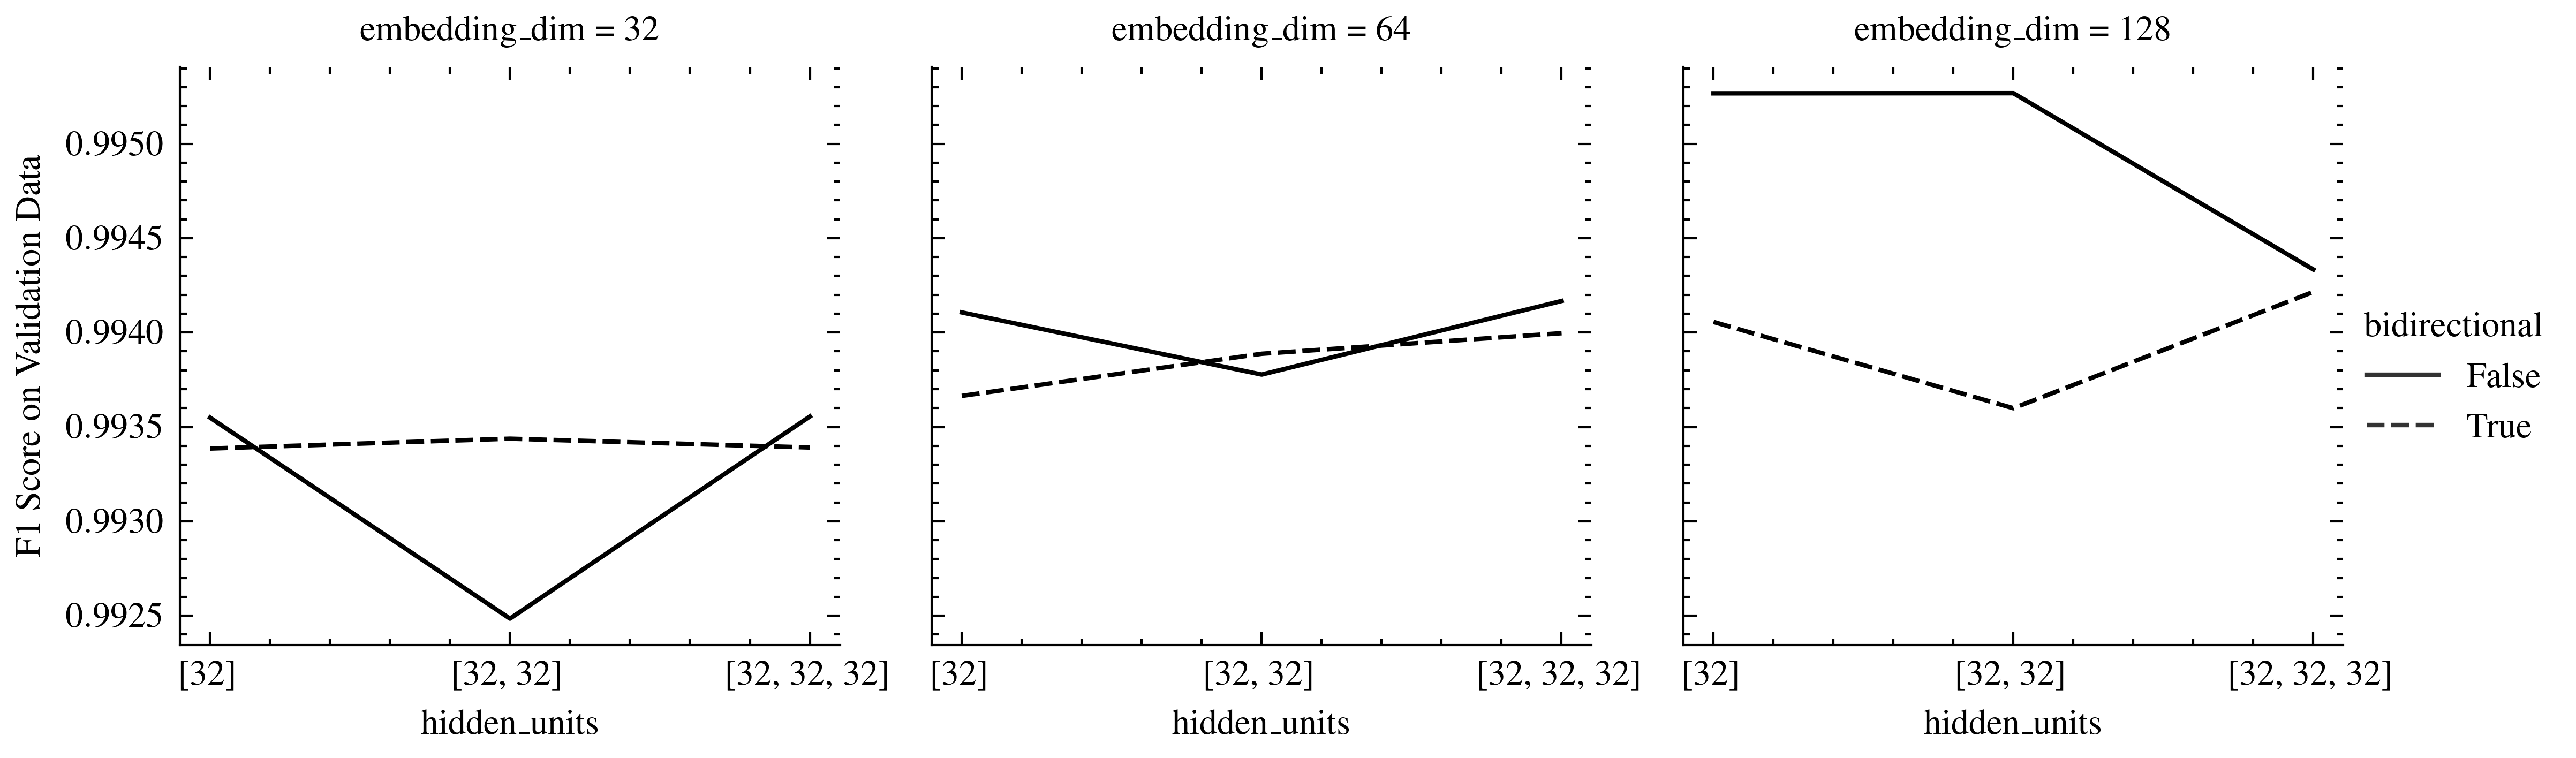
\includegraphics[width=.5\textwidth]{image/lstm_hyperparameter_tuning.png}
  \caption{LSTM hyperparameter combinations result}
  \label{fig:lstm-tuning}
\end{figure}

\begin{figure}[!h]
  \centering
  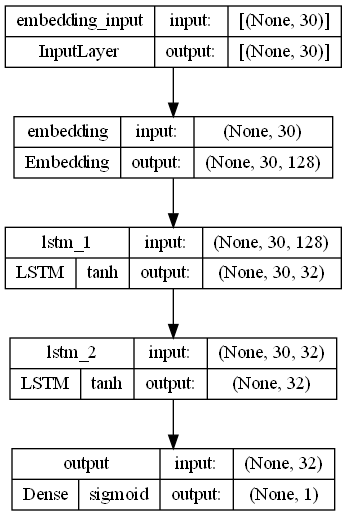
\includegraphics[width=.26\textwidth]{image/lstm_best_model_architecture.png}
  \caption{Best model architecture for LSTM}
  \label{fig:best-model-architecture}
\end{figure}

\begin{figure}[!h]
  \centering
  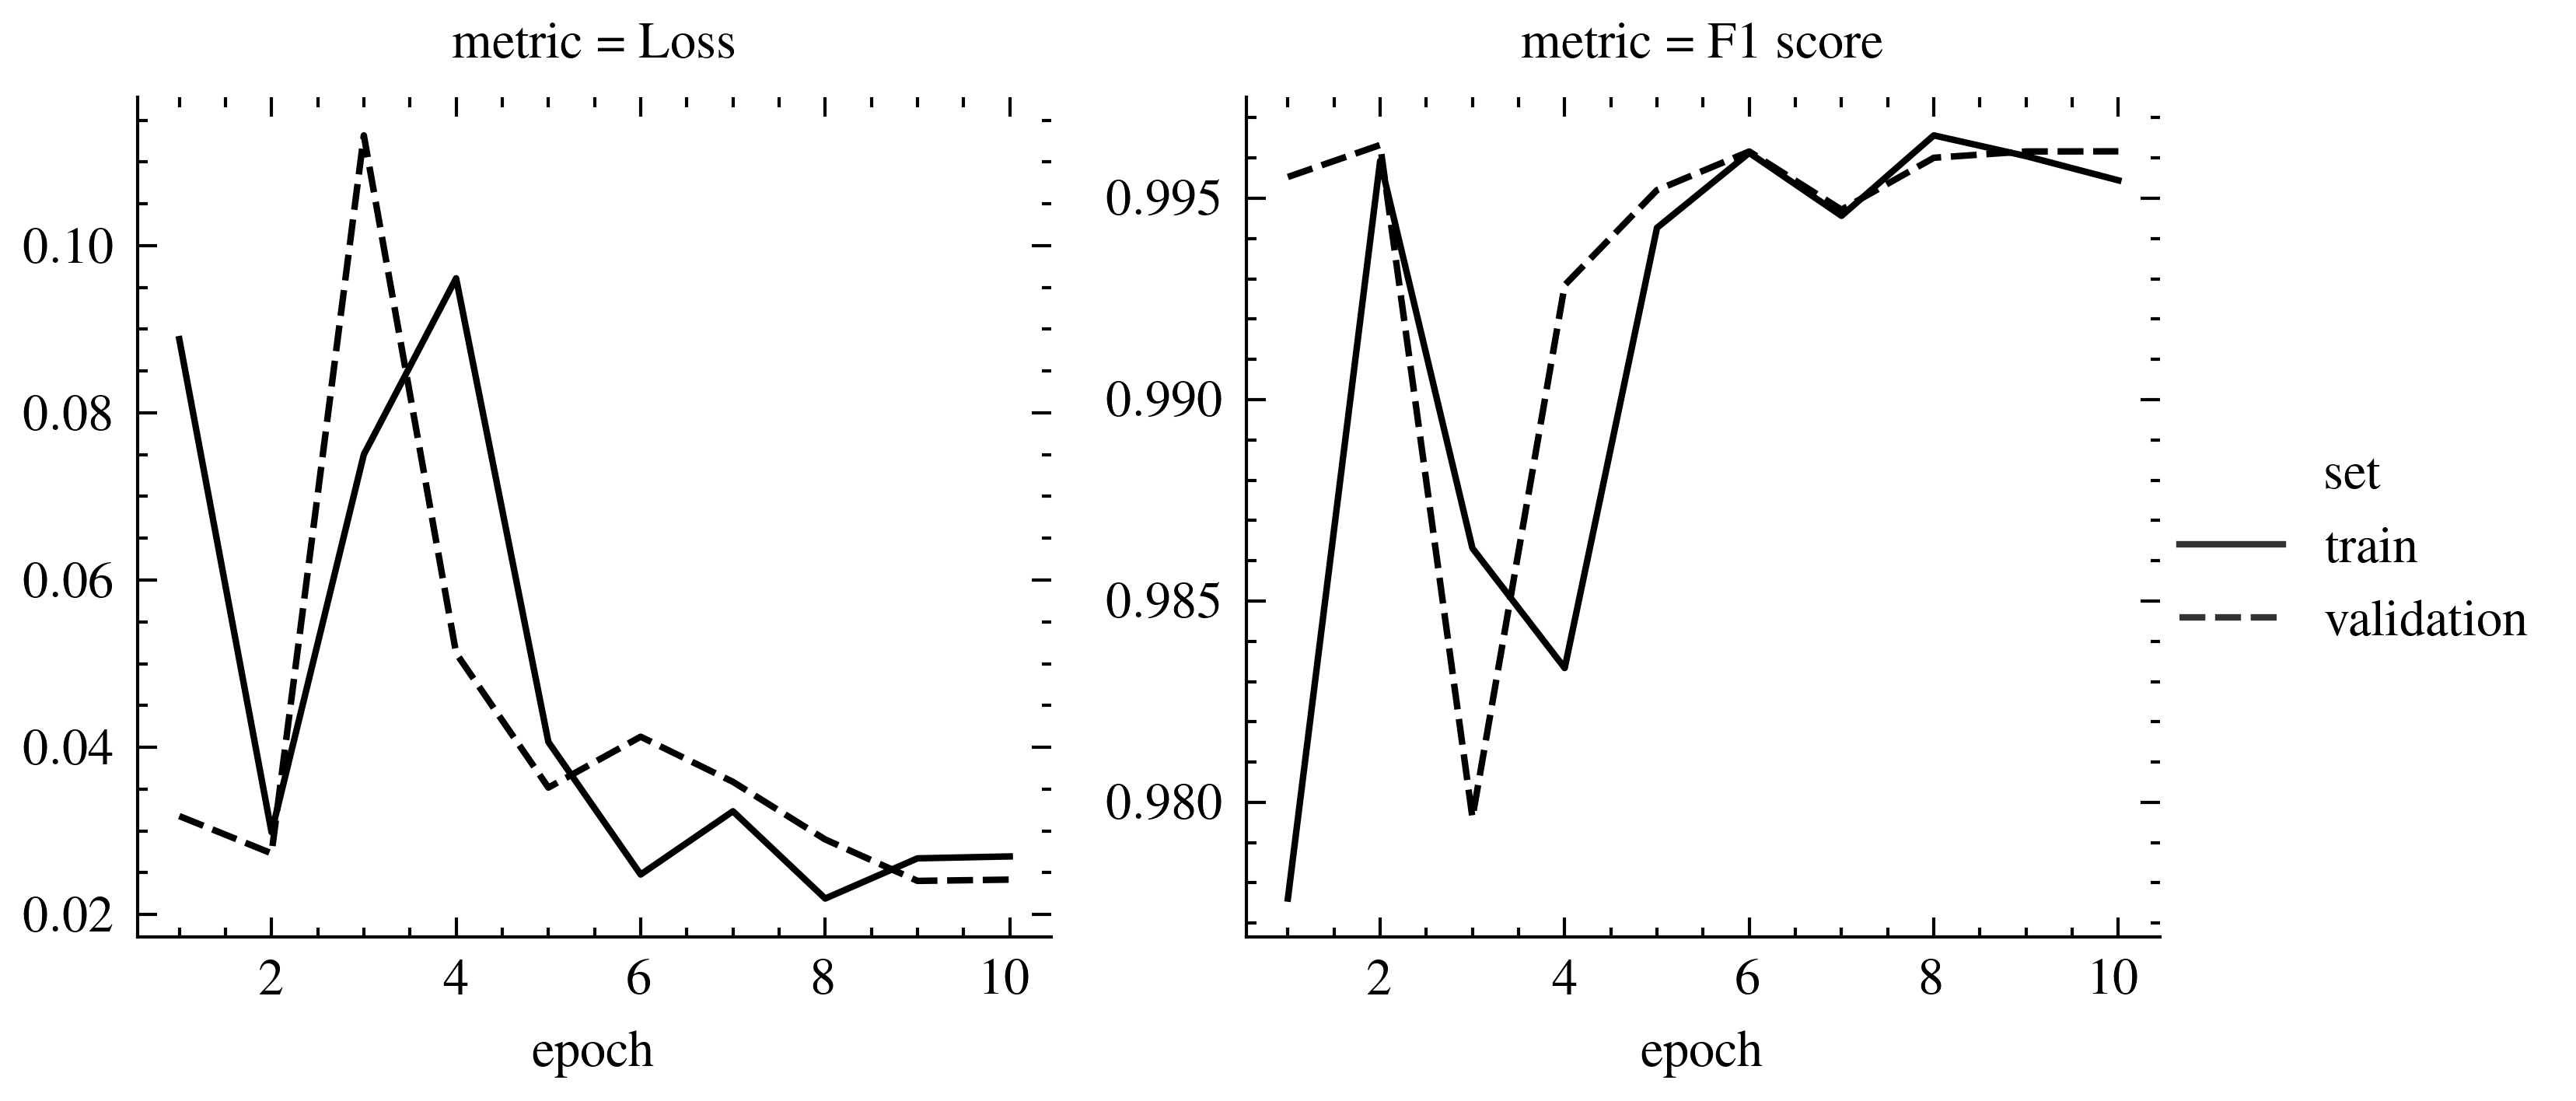
\includegraphics[width=.5\textwidth]{image/lstm_best_model_performance_per_epoch_without_acc.png}
  \caption{Performance per epoch for LSTM}
  \label{fig:lstm-performance-per-epoch}
\end{figure}

\subsection{Comparison with machine learning algorithms}
\label{subsec:comparison-with-machine-learning}
\par The LSTM model in Figure \ref{fig:best-model-architecture} is then compared with the ten classical machine learning algorithms in terms of F1 score and prediction time, measured in milliseconds per query. In Figure \ref{fig:ml_and_lstm_time_vs_f1}, the model in the lower-right region is preferred since it has a higher F1 score and faster prediction time. In the end, we still chose LSTM as our model in the prediction phase since it achieves the best F1 score and the prediction time is relatively fast compared to other algorithms.

\begin{figure}[!h]
  \centering
  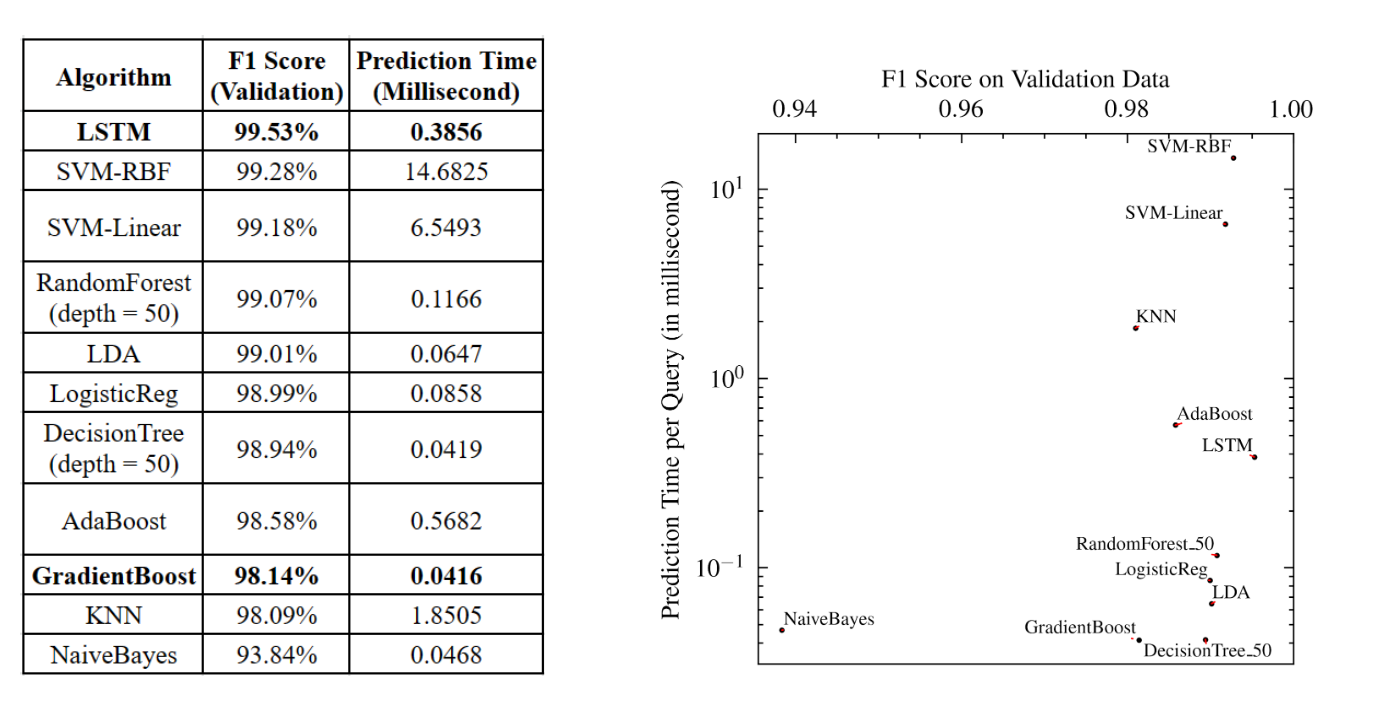
\includegraphics[width=.5 \textwidth]{image/ml-compare.png}
  \caption{Prediction time versus F1 score on 11 different algorithms}
  \label{fig:ml_and_lstm_time_vs_f1}
\end{figure}

\subsection{Comparison of the one-step and two-step approach}
\label{subsec:comparison-two-step}
\par Table \ref{tab: one-step-vs-two-step} shows the comparison between our one-step and two-step approaches. The one-step approach applies only keyword filtering or model prediction separately. Meanwhile, the two-step approach is done by combining both approaches. The keyword filtering using a blacklist help the model prediction to increase the final F1 score on test data by 0.11\%. Although insignificant, it still proves that using a two-step approach is better than only using one of either approach.

\begin{table*}[!htp]\centering
\caption{One-step versus two-step approach}\label{tab: one-step-vs-two-step}
\scriptsize
\begin{tabular}{lrrrrr}\toprule
\multirow{}{}{\textbf{Prediction Approach}} &\multicolumn{2}{c}{\textbf{Accuracy}} &\multicolumn{2}{c}{\textbf{F1 Score}} \\\cmidrule{2-5}
&\textbf{Train} &\textbf{Test} &\textbf{Train} &\textbf{Test} \\\midrule
Only model prediction &99.65\% &99.27\% &99.52\% &99.01\% \\
Only keyword filtering &63.29\% &63.31\% &0.59\% &0.61\% \\
Two-step prevention (Proposed method) &99.7\% (+0.05\%) &99.35\% (+0.08\%) &99.59\% (+0.07\%) &99.12\% (+0.11\%) \\
\bottomrule
\end{tabular}
\end{table*}

\subsection{Comparison with related work}
\label{subsec:comparison-two-step}

\par As shown in Table \ref{tab:comparison-with-related-works }, our proposed design demonstrates strong predictive capabilities and is competitive with state-of-the-art models like LSTM and CNN. While our proposed approach does have slightly lower performance than the LSTM in \cite{8877739}, it's worth noting that the LSTM in \cite{8877739} (DS5) was trained on a dataset with a different ratio of positive to negative samples (5:5 ratio). Specifically, SQLi detection performs best when the ratio of positive to negative samples is between 4:5 and 5:5, and its performance decreases as the proportion of positive samples increases. For the CNN Comparison, despite the slight disadvantage in performance, our proposed design still outperforms the CNN model in \cite{8616823} by a factor of 10 in terms of prediction time.

\begin{table}[!htp]\centering
\caption{Comparison with related work}\label{tab:comparison-with-related-works }
\scriptsize
\begin{tabular}{lrrrrr}\toprule
\multirow{}{}{\textbf{Prediction Approach}} &\multicolumn{2}{c}{\textbf{Accuracy}} &\multicolumn{2}{c}{\textbf{F1 Score}} \\\cmidrule{2-5}
&\textbf{Train} &\textbf{Test} &\textbf{Train} &\textbf{Test} \\\midrule
Dense Neural Network \cite{SQLiDataset} &- &97.73\% &- &96.36\% \\
Ensemble Boosted Trees \cite{8959617} &93.70\% &- &- &- \\
Support Vector Machine \cite{7987433} &- &98.60\% &- &98.50\% \\
LSTM (DS1) \cite{8877739} &- &93.74\% & &92.99\% \\
LSTM (DS5) \cite{8877739} &- &99.58\% &- &99.76\% \\
CNN \cite{8616823} &- &99.93\% &- &99.95\% \\
\textbf{Two-step prevention (ours)} & \textbf{99.70\%} & \textbf{99.35\%} & \textbf{99.59\%} & \textbf{99.12\%} \\
\bottomrule
\end{tabular}
\end{table}
  % Ubah judul dan label berikut sesuai dengan yang diinginkan.
\section{Conclusion and Future Works}
\label{sec:conclusion}
\par We have proposed a two-step prevention for SQLi, using a blacklist for keyword filtering and the LSTM model. LSTM performed better than the other ten classical machine learning approaches (99.53\% F1 score on validation data) but it requires more predicting time. Even so, we can consider the model to be relatively fast (under 1 millisecond per query). With the additional use of keyword filtering, the predictive performance is increased but insignificant. Our approach competes well with state-of-the-art approaches. We also have developed a simple web application for a login use case to make our proposed method accessible to testers.

\par To further enhance the effectiveness of our approach, we can implement explainable AI using LIME (Local Interpretable Model-agnostic Explanations) in the backend system. This would provide administrators with more detailed information when an attack is detected. Currently, our proposed system relies solely on a blacklist for keyword filtering. However, we can also consider using a whitelist approach, such as a regex email filter, to reduce false positives in our SQLi detection. This would provide an additional layer of protection and improve the performance of our system.


  % Menampilkan daftar pustaka dengan format IEEE
  \bibliographystyle{IEEEtranN}
  \bibliography{pustaka/pustaka.bib}

  % Menyeimbangkan bagian akhir di kedua kolom
  \balance

\end{document}
